\documentclass[a4paper, UTF8]{ctexart}

\usepackage{amsmath}
\usepackage{amssymb}
\usepackage{biblatex}
\usepackage{graphicx}
\usepackage[hidelinks]{hyperref}
\usepackage{listings}
\newtheorem{proposition}{命题}
\DeclareMathOperator{\sgn}{\mathrm{sgn}}
\lstset{
    basicstyle=\small\tt,
    numbers=left
}
\addbibresource{num2sqrts.bib}

\title{将一个浮点数转换为两根式之和的最简算法}
\author{郑}

\begin{document}
\maketitle

\section{引言}
一些数值计算器在计算分式、根式以及角度时会返回类似$\dfrac{\pi}{3}$或$\dfrac{2\sqrt{2}}{3}$的结果而非浮点数. 它们同样也会显示$1+\sqrt{2}$和$\dfrac{\sqrt{2}+\sqrt{3}}{2}$. 前两者可通过简单的数学运算得出,但是后面两个涉及到了加法运算. 如果我们想分别求出$\dfrac{\sqrt{a}+\sqrt{b}}{c}$中的$a$、$b$和$c$,最简单的方法是使用三重for循环,但这是效率非常低的方法. 我们是否可以设计一种方法高效的解决上述问题?这就是我创作这篇文章的目的:介绍一个新的算法将一个浮点数转换为两根式之和.

\section{理论}
我们先讨论没有分母的形式. 为叙述方便,先定义一函数\[S(x,y)=\sgn(x)\sqrt{|x|}+\sgn(y)\sqrt{|y|} \quad\mbox{其中}x,y\in\mathbb{Z}\]如果我们仅仅知道浮点数$n=S(a,b)$,我们可以使用一些数学技巧和仅一个while循环求出$a$和$b$,而不是使用双重for循环. 简而言之,我们的目的是找到$S^{-1}:\mathbb{R}\to\mathbb{Z}^2$.

当然,使用既定公式求出$S^{-1}(x)$是不可能的. 唯一可行的途径是穷举搜索. 使用不同的方法进行穷举都可以获得正确的结果,但效率的差异可能是巨大的. 我将介绍一种效率较高的方法. 先从以下真命题开始:
\begin{proposition}
    若已知两数之和$a+b$,以及它们的均值$c=\dfrac{a+b}{2}$,那么$|c-a|=|c-b|$. 
\end{proposition}
根据上述命题,若已知$n=S(a,b)$, 我们可以从$\dfrac{n}{2}$开始向$\pm\infty$方向搜索. 一旦确定了$a$就可以知道唯一的$b$,最后我们仅仅需要一些额外的判断就能得知它们是否为所求.

当然,使用$\dfrac{n}{2}$作为初始值是不合适的,因为我们需要的结果是两个整数. 使用截尾取整后的$\left(\dfrac{n}{2}\right)^2$更适合.

不过,我们可以计算出$\left(\dfrac{\sqrt{100}+\sqrt{101}}{2}\right)^2\approx100.499$,它会舍入到100,这样的设计也是有漏洞的. 但是,有如下极限\[\lim_{x\to+\infty}\left(\frac{\sqrt{x}+\sqrt{x+1}}{2}\right)^2-x=\frac{1}{2}\]它表示函数$f(x)=\left(\dfrac{\sqrt{x}+\sqrt{x+1}}{2}\right)^2$可以近似成$x+\dfrac{1}{2}$.

这样,即使$S(a,b)$中的$a$、$b$的差值很小我们也能分别求出它们。

根据以上的分析,我们可以这样计算初始值
\[
    start(n)=
    \begin{cases}
        \lfloor(\frac{n}{2})^2\rfloor+\frac{1}{2}  &n>0 \\
        -\lfloor(\frac{n}{2})^2\rfloor-\frac{1}{2} &n<0
    \end{cases}
\]

为了书写方便,下面规定一负数的平方根是其绝对值平方根的相反数.

已知$n=S(a,b)$,初始值$start=start(n)$,令$step=0.5$并找到第一个数字\[\alpha=start-step\]接着就能求出第二个数字\[\beta=\frac{n}{2}-|\sqrt{a}-\frac{n}{2}|\]$\beta$必须是一个整数,我们接下来还要做如下操作\[\beta=\sqrt{\sgn(\beta)\mathrm{round}(\beta^2)}\]其中\verb|round|表示舍入到最近的整数.

如果$|\sqrt{\alpha}+\sqrt{\beta}-n|\leq\varepsilon$,其中$\varepsilon$表示一个很小的数,那么$\alpha$和$\beta$就是所求的$a$和$b$. 否则我们令$step=step+1$继续向正无穷方向搜索.

\section{实现}
以下是本算法的Python实现.

\begin{lstlisting}[language=python, name=example1]
import math

def num2sqrts(n, max_num=1000):
    if n >= 0:
        mid = math.floor((n / 2) ** 2) + 0.5
    elif n < 0:
        mid = math.ceil(-(n / 2) ** 2) - 0.5
    fsqrt = lambda n: math.copysign(math.sqrt(math.fabs(n)), n)
    actual_mid = n / 2
    t = 0.5
    while True:
        a = fsqrt(mid + t)
        d = math.fabs(a - actual_mid)
        b = actual_mid - d
        b = fsqrt(math.copysign(round(b ** 2), b))
\end{lstlisting}
理论上来说,该算法可以一直执行,直到找到正确的结果. 但是考虑到实际情况,我们必须有一个停止条件.
\begin{lstlisting}[language=python, name=example1]
        if abs(a ** 2) > max_num or abs(b ** 2) > max_num:
            return
        if math.isclose(a + b, n):
            return int(round(math.copysign(a ** 2, a))), \
                int(round(math.copysign(b ** 2, b)))
        t += 1
\end{lstlisting}
最后,函数\verb|num2sqrts|长度为2的元组作为结果. 若返回\verb|None|,这表示程序没有找到正确的结果.

\begin{figure}[tp]
    \centering
    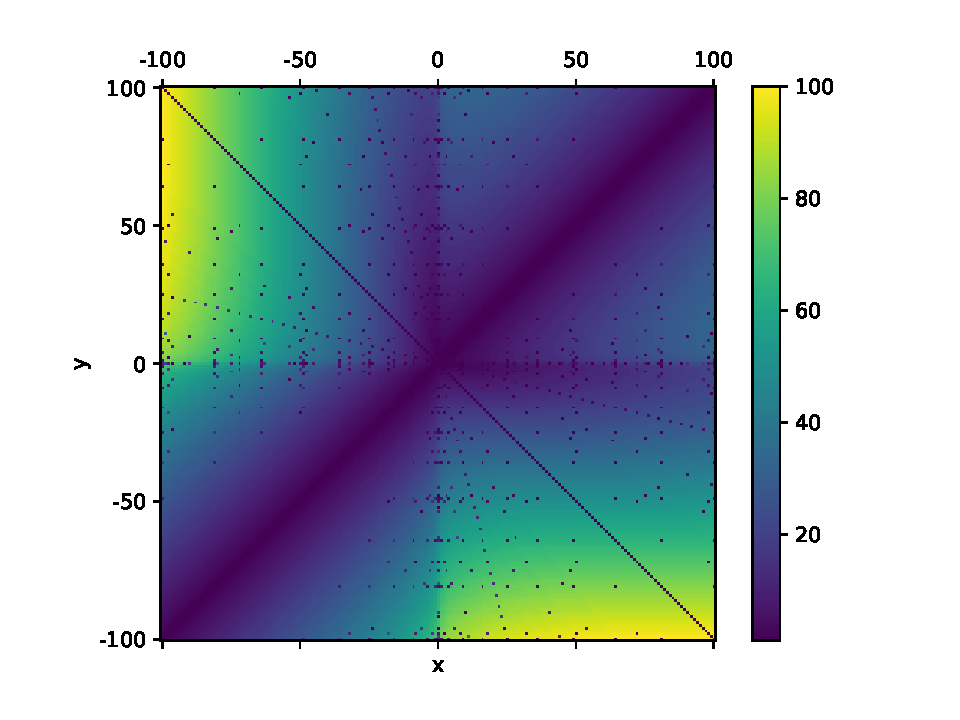
\includegraphics[width=0.8\linewidth]{perform.pdf}
    \caption{算法的表现}
    \label{fig:perform1}
\end{figure}

为了展示算法的表现,我令$-100\leq x\leq100$和$-100\leq y\leq100$,接着记录算法需要多少次循环可求出$S(x,y)$中的$x$和$y$,最后把它们以不同的颜色标识(见图 \ref{fig:perform1}). 可见,当$x$、$y$之差越大时,需要执行更多次的循环.

不过当我们运行如下(或类似)语句时
\begin{lstlisting}[language=python]
num2sqrts(2 * math.sqrt(123))
\end{lstlisting}
函数返回\verb|(492, 0)|,循环执行了438次. 不过$2\sqrt{123}$这个结果可以以一个更简单的算法找到,故我将图 \ref{fig:perform1} 中一、三象限对角线上的值全部赋值为1.

最后,我将阐述分母不为1的情况. 再寻找一个算法显得异常低效,我们完全可以穷举分母.
\begin{lstlisting}[language=python, name=example2]
def num2sqrts2(value):
    for n in range(1, 100):
        if (ret := num2sqrts(value * n)) is not None:
            return *ret, n
\end{lstlisting}
毫无疑问,穷举的范围可以随意扩大(在这里是1--99). 相应的,算法运行的时间也有可能会增加.

\section{比较}
% normal_one(34.35s) vs num2sqrts(0.14): 251.22
使用嵌套的for循环(我称其为 \verb|normal_one| 算法)同样也可以求出两根式之和.

mpmath\cite{mpmath}有\verb|mpmath.identify|函数也可以将浮点数转换为数学表达式,且支持更复杂的形式:
\begin{lstlisting}[language=python]
>>> import mpmath, sympy
>>> s = mpmath.identify(mpmath.sqrt(2) + mpmath.sqrt(3))
>>> s
'sqrt(((10+sqrt(96))/2))'
>>> sympy.simplify(s)
sqrt(2*sqrt(6) + 5)
\end{lstlisting}
但是,参照上述的运行结果,问题则变成了化简双重根号,就需要编写化简双重根号的程序了,这里不再赘述.

\section{结论}
在这篇文章中,我介绍了 \verb|num2sqrts| 算法,它可以将一些浮点数转换为与之相等的、具有特定形式的数学表达式. 同时,该算法简单、快速,适合应用在科学计算器中.

\printbibliography[title={参考文献}]

\end{document}
